% Chapter 7

\chapter{Background Processes} % Chapter title

\label{ch:background_processes} 

%----------------------------------------------------------------------------------------

This analysis is fundamentally a search for \ac{SUSY} in events with two leptons whose invariant mass (\mll) is consistent with a $Z$ boson. Additional event selections are made to reduce \ac{SM} processes relative to potential \ac{SUSY} processes, defined by simplified models discussed in \autoref{sec:simplified_models}. These models include the production of strongly-charged, high-mass particles, which results in events with jets and high \HT, the scalar sum of the \pt of all jets and the two leading leptons in the event. These $R$-parity conserving \ac{SUSY} models also produce decay chains that terminate with a stable, electrically neutral particle, which produces \MET when it passes through \ac{ATLAS} without detection. Each of these features can help isolate these signal events from \ac{SM} backgrounds. To understand what cuts would optimize the sensitivity of the search, it is essential to first understand what these \ac{SM} backgrounds are. 

\begin{centering}
\begin{figure}[bth]
\myfloatalign
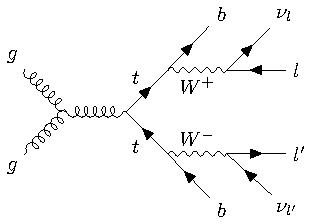
\includegraphics[width=.70\linewidth]{feynman/ttbar.pdf}
\caption{An example Feynman diagram of \ttbar production and decay.}
\label{fig:ttbar}
\end{figure}
\end{centering}

\paragraph{Top-antitop (\ttbar)} production is the largest background for this search because it often precisely mimics the signature expected from the signal process. \autoref{fig:ttbar} shows a Feynman diagram of this process, which results in two jets, leptons, and neutrinos, which are seen in the detector as \MET. Thus, \ttbar events naturally have high \MET and \HT, jets, and leptons from two different $W$ boson decays, which may coincidentally form an invariant mass consistent with a $Z$ boson. Separating these events from signal processes is very difficult, but some steps can be taken to reduce their impact. The leptons resulting from \ttbar don't originate from the same parent particle, so their invariant mass distribution is very broad compared to processes involving leptons from $Z$ bosons. As a consequence, reducing the width of the \mll~window used to identify $Z$-boson candidates can help to reduce this background. Additionally, for sparticles with a higher mass than that of the top quark, the \HT distribution will typically be larger for signal models than for \ttbar. Though the two \HT distributions overlap significantly for most signal models, a high cut on \HT can help to reduce the \ttbar background relative to a potential signal.  

\begin{centering}
\begin{figure}[bth]
\myfloatalign
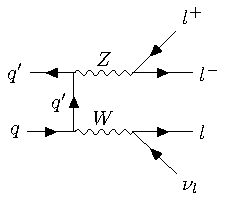
\includegraphics[width=.70\linewidth]{feynman/diboson.pdf}
\caption{An example Feynman diagram of the production and decay of a WZ event.}
\label{fig:diboson}
\end{figure}
\end{centering}

\paragraph{diboson ($VV$)} production is the next leading background. These processes have lower cross-sections than that of \ttbar, but they can also produce events with topologies very similar to signals. Diboson events can contain real $Z$ bosons and their dilepton invariant mass will peak on-$Z$ like a signal. In addition, in events like \autoref{fig:diboson}, an additional $W$ boson can decay to another lepton and a neutrino, producing \MET. The pictured process can occur with associated jets due to initial state radiation, but each additional jet reduces the process's rate by a factor of $\alpha_s$. If the $W$ boson in this figure instead decayed to two jets, which occurs about twice as often as the pictured decay, there would be no true \MET from a neutrino. Thus, introducing a requirement that the signal region include both high amounts of \MET and at least two jets can very effectively reduce the contribution from both these scenarios. A veto on a third lepton could also be used to reduce the contribution from events with $W\rightarrow \ell \nu$ decays, but, depending on the signal model considered, this veto can also decrease signal acceptance. Since the branching ratio for this process is relatively small, the potential reduction in signal acceptance is deemed more important, and a third lepton veto is not used in this analysis. 

\begin{centering}
\begin{figure}[bth]
\myfloatalign
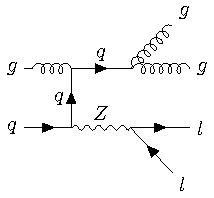
\includegraphics[width=.70\linewidth]{feynman/zjets.pdf}
\caption{An example Feynman diagram of the production and decay of a \dyjets event.}
\label{fig:zjets}
\end{figure}
\end{centering}

\paragraph{\dyjets} processes are very common but, as shown in \autoref{fig:zjets}, don't typically produce any true \MET. The exception is $Z\rightarrow\tau\tau$ events, which contain \MET because the $\tau$ leptons decay within the detector, and these decays include $\tau$ neutrinos. However, only about 1/3 of $\tau$ decays produce an electron or muon, and even if two leptons are created in an event, they will typically not reconstruct a $Z$ mass due to the energy lost to the neutrinos. For the purposes of this analysis, \textit{lepton} refers only to electrons and muons, and excludes these more complicated $\tau$ events. A high \HT cut helps reduce the \dyjets background, but this process can occur with initial state radiation, producing events with large amounts of hadronic activity. \MET is the most powerful variable for reducing $Z\rightarrow\mu\mu$ and $Z\rightarrow ee$ events, because though events with mismeasured jets or leptons can fake \MET, mismeasurements drastic enough to produce hundreds of \gev~of \met are rare. In addition, events with substantially mismeasured leptons often have \mll~values that are inconsistent with a $Z$ boson, and so a fraction of \dyjets events that do pass a \MET threshold can be excluded nonetheless. 

Other processes can contribute to the \ac{SM} background at lower rates. Processes similar to \dyjets but with a $W$ boson instead of a $Z$ have real \MET from leptonic $W$ decays, but only one lepton. However, a fake or non-prompt lepton can cause these events to look very similar to simulated signals. Single top production can occur in association with a $W$ boson, which produces signatures similar to \ttbar, but with fewer jets.  Additionally, there are \textit{rare top} processes such as \ttbar production in association with $W$ or $Z$ bosons, which are event more difficult to separate from signal events than \ttbar due to the presence of a genuine $Z$ boson, the increased \met from $W$ decays, and the larger amounts of hadronic activity.

Several of these backgrounds are grouped together and referred to as \textit{\aclu{FS}} (\acs{FS}) processes. These include any processes that produce pairs of leptons with uncorrelated flavor in the final state. In this analysis, the largest \ac{FS} background is \ttbar, with additional contributions from $WW$, $Wt$, and $Z\rightarrow\tau\tau$ events. In these processes, each lepton comes from the decay of a different particle. In the case of \ttbar, the two top quarks decay to $W$ bosons, which each produce a lepton in their decays, as shown in \autoref{fig:ttbar}. Consequently, these leptons' flavors are correlated with the flavor of the neutrino that results from the same boson's decay, but not with one another.

\section{Data and Monte Carlo Samples} 

This analysis uses data collected by the \ac{ATLAS} detector from $pp$ collisions at a center-of-mass energy of 13 \tev~in 2015 and 2016, corresponding to a total luminosity of 14.7 fb$^{-1}$. The data collected use a combination of unprescaled single and dilepton triggers, discussed in greater detail in \autoref{sec:trig_strategy}. The triggers targeting the lowest \pt ranges are fully efficient for pairs of leptons with \pt of at least 20 \gev. In addition, photon events are collected for use in a control region using both prescaled and unprescaled triggers, with the lowest trigger threshold at 35 \gev~in 2015 and 20 \gev~in 2016. 

\ac{MC} samples are generated for each background process that appears in the signal and validation regions. \autoref{tab:MC} details the generators used to produce each sample, and more information can be found in \autoref{sec:MC_gen}. These simulated background events, in conjunction with the simulated signal discussed in \autoref{sec:simplified_models}, are used to determine approximate sensitivities of the search and optimize signal regions. The background \ac{MC} also provides a valuable cross-check for many of the data-driven background estimates discussed in \autoref{ch:backgrounds}, and in the case of rare top and some diboson events, provides the primary estimate of the background.

\begin{sidewaystable*}[ht]
\begin{center}
\caption{Simulated background event samples used in this analysis with the corresponding matrix element and parton shower generators,
cross-section order in $\alpha_{\text{s}}$ used to normalize the event yield, underlying-event tune and PDF set.
}
\scriptsize
\begin{tabular}{l c c c c c }
\hline
Physics process &  Generator  & Parton & Cross section & Tune & PDF set\\
                &             & Shower &              &      & \\
%\hline\hline
\noalign{\smallskip}\hline\noalign{\smallskip}
$t\bar{t}+W$ and $t\bar{t}+Z$~\cite{ATL-PHYS-PUB-2016-005,Garzelli:2012bn}& {\sc MG5\_aMC@NLO}        & {\sc Pythia} 8.186 & NLO \cite{Campbell:2012,Lazopoulos:2008} & {\sc A14} & NNPDF23LO\\
$t\bar{t}+WW$~\cite{ATL-PHYS-PUB-2016-005}      & {\sc MG5\_aMC@NLO}          & {\sc Pythia} 8.186 & LO \cite{Alwall:2014hca} & {\sc A14}  &  NNPDF23LO\\
$t\bar{t}$~\cite{ATL-PHYS-PUB-2016-004}         & {\sc Powheg Box v2} r3026   & {\sc Pythia} 6.428 & NNLO+NNLL \cite{ttbarxsec1,ttbarxsec2}          &\sc{Perugia2012}     &NLO CT10\\
Single-top ($Wt$)~\cite{ATL-PHYS-PUB-2016-004}  & {\sc Powheg Box v2} r2856   & {\sc Pythia} 6.428 & Approx. NNLO \cite{Kidonakis:2010b}& \sc{Perugia2012}    &NLO CT10 \\ 
$WW$, $WZ$ and $ZZ$~\cite{ATL-PHYS-PUB-2016-002} & \sherpa\ 2.1.1 & \sherpa\ 2.1.1 & NLO \cite{diboson1,diboson2} & \sherpa\ default & NLO CT10 \\
%$WZ$ and $ZZ$~\cite{ATL-PHYS-PUB-2016-002} &&& \\ 
$Z/\gamma^{*}(\rightarrow \ell \ell)$ + jets~\cite{ATL-PHYS-PUB-2016-003}& \sherpa\ 2.1.1           & \sherpa\ 2.1.1  &NNLO \cite{DYNNLO1,DYNNLO2}       & \sherpa\ default     &NLO CT10\\
\gjets & \sherpa\ 2.1.1 & \sherpa\ 2.1.1 & LO~\cite{sherpa} & \sherpa\ default & NLO CT10 \\
$V(=W,Z)\gamma$ & \sherpa\ 2.1.1 & \sherpa\ 2.1.1 & LO~\cite{sherpa} & \sherpa\ default & NLO CT10 \\
signal & {\sc MG5\_aMC@NLO} & {\sc Pythia} 8.186 & NLO & A14 & NNPDF23LO\\
\noalign{\smallskip}\hline\noalign{\smallskip}
\end{tabular}
\label{tab:MC}
\end{center}
\end{sidewaystable*}
